\documentclass[9pt,twocolumn,twoside]{osajnl}
%% Please use 11pt if submitting to AOP
% \documentclass[11pt,twocolumn,twoside]{osajnl}

\journal{ol} % Choose journal (ao,jocn,josaa,josab,ol,optica,pr)

%See template introduciton for guidance on setting shortarticle option
\setboolean{shortarticle}{true}
% true = letter/tutorial
% false = research/review article
% (depending on journal)


\usepackage{lineno}
\linenumbers


\title{Analysis of EEG cortical recordings}


\author{Khomutov, Grigoriev, Volos, Gordiychuk}


\begin{abstract}
We have performed spectral analysis on 6-channel EEG recordings from 4 subjects, recorded during concentration or meditation, with the eyes open or closed. 

\end{abstract}


\begin{document}

\maketitle

\section{Processing of signals}

Figure \ref{fig:false-color} shows a raw O1 - electrode $\alpha$-signal.

\begin{figure}[htbp]
\centering
\fbox{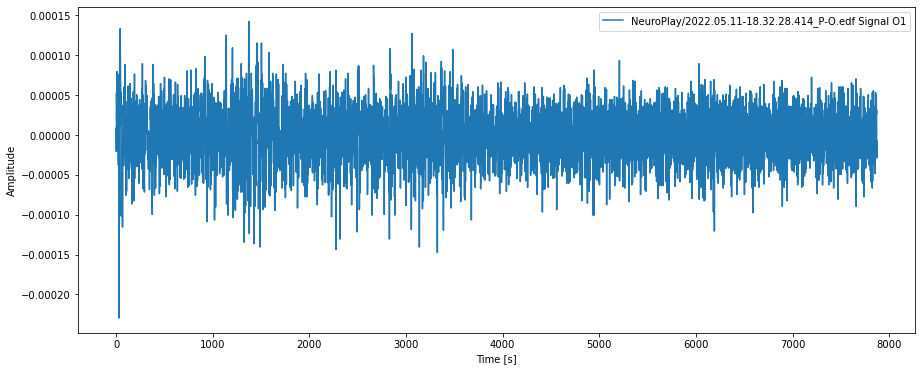
\includegraphics[width=\linewidth]{NP1.png}}
\caption{Raw signal}
\label{fig:false-color}
\end{figure}

\begin{figure}[htbp]
\centering
\fbox{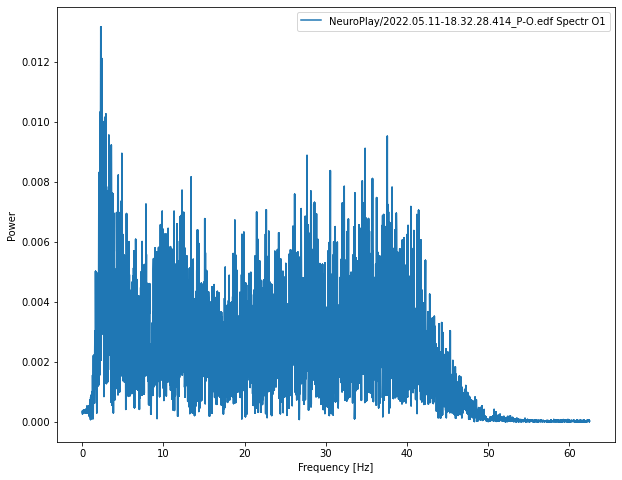
\includegraphics[width=\linewidth]{image_2022-05-12_16-00-15(2).png}}
\caption{Raw spectrum}
\label{fig:false-color}
\end{figure}

To eliminate the noise in our signal, we will use the Hilbert Transformation (HT). HT is widely used in signal demodulation. When mechanical faults occur, the collected vibration signals are generally modulated. \\
Therefore, signal demodulation is able to separate the carrier component and modulation component. We can perform the same procedure with the experimentally obtained spectrum.

\begin{figure}[htbp]
\centering
\fbox{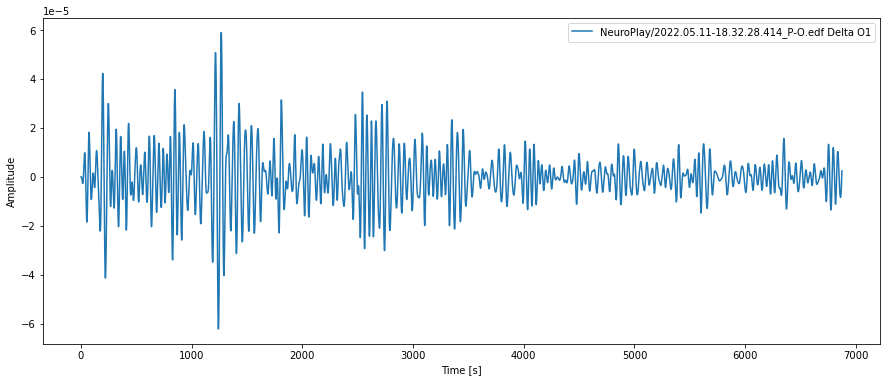
\includegraphics[width=\linewidth]{image_2022-05-12_16-00-15(1).png}}
\caption{Transformed signal}
\label{fig:false-color}
\end{figure}




\begin{figure}[ht!]
\centering
\fbox{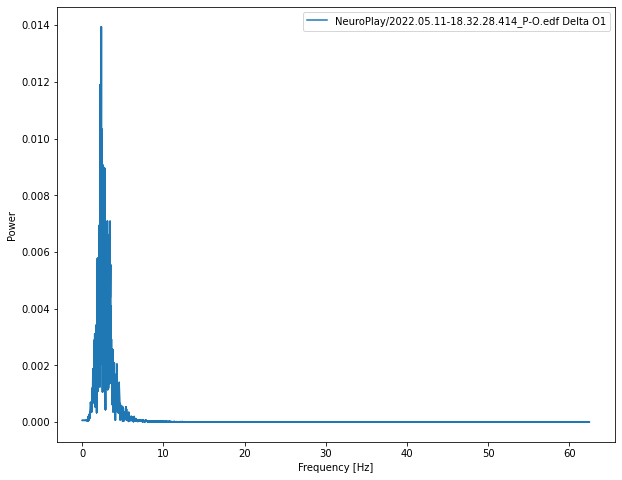
\includegraphics[width=\linewidth]{image_2022-05-12_16-00-15(3).png}}
\caption{Transformed spectrum}
\label{fig:false-color}
\end{figure}

\section{Open vs. Closed eyes}

To compare $\alpha, \beta, \gamma, \delta, \theta$ rhythms between open and closed eyes, we used scalp maps that show us the distribution of excitation in the brain. 

\par Generally $\alpha$-waves induce feelings of calm, increase creativity, and enhance your ability to absorb new information.
\par $\beta$-waves are involved in conscious thought and logical thinking and tend to have a stimulating effect. Having the right amount of beta waves allows us to focus.
\par High $\beta$-waves occur when a person is excited or anxious. They also occur while experiencing something new or having complex thoughts. 
\par $\gamma$-waves are also associated with high levels of thought and focus.

A person who has taken time off from a task and begins to daydream is often in a $\theta$ brainwave state. Theta waves are the most prominent in situations where tasks become so automatic that you can mentally disengage from them. We get to mostly $\delta$ waves as we go to sleep.

\begin{figure}[htbp]
\centering
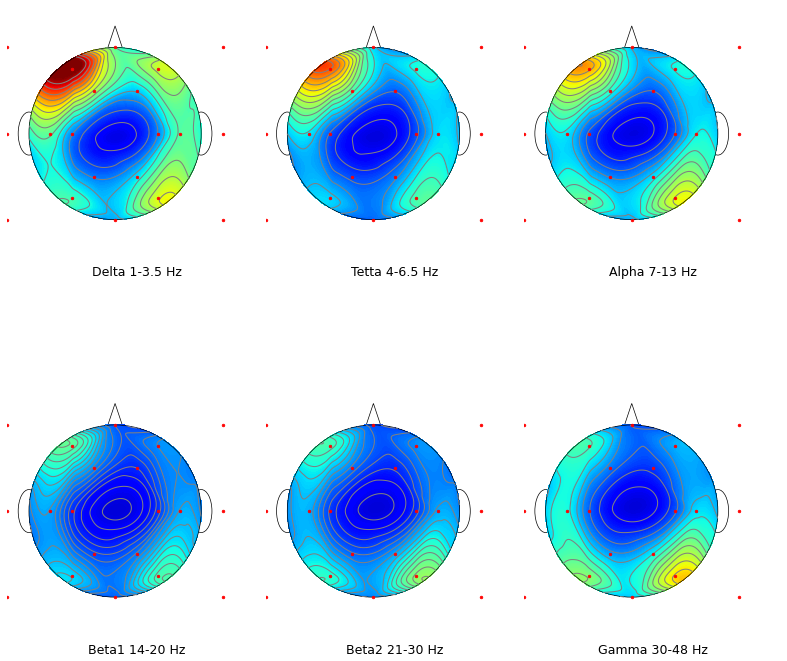
\includegraphics[width=\linewidth]{image_2022-05-12_17-41-41.png}
\caption{Open eyes}
\label{fig:false-color}
\end{figure}

\begin{figure}[htbp]
\centering
\fbox{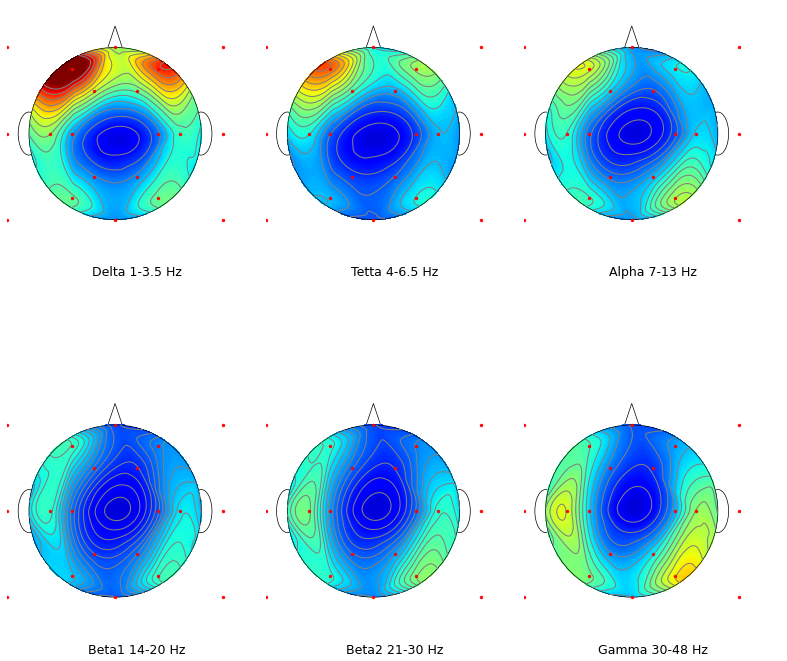
\includegraphics[width=\linewidth]{image_2022-05-12_17-40-45.png}}
\caption{Closed eyes}
\label{fig:false-color}
\end{figure}

 As we can see from Fig. 5 and Fig.6, $\alpha$ waves were more active when the subject had their eyes closed. This can result from a person feeling calmer with their eyes closed. $\beta$-waves were more active in the temporal lobes when the eyes were closed, and in the frontal and occipital lobes when the eyes were open. This is expected as with closed eyes the subject would be receiving the most information auditory and with open eyes visually. Having eyes open could also increase focus, which can explain the beta waves increase in the frontal lobe. Slower $\gamma$, $\delta$ and $\theta$ waves increase with eyes closed are also expected as they are related with less interference with the outside world.



\section{Metrics' analysis}

Three differents metrics were evaluated via provided formulas:
\begin{equation}
    Concenration = \frac{TP_{\beta_1} + TP_{\beta_2}}{TP_{\theta}},
\end{equation}
\begin{equation}
    Meditation = \frac{TP_{\alpha}}{TP_{0}},
\end{equation}
\begin{equation}
    Well\text{-}being = \frac{TP_{F_4}}{TP_{F_3}},
\end{equation}
where $TP_i$ stands for TotalPower - the sum of squared amplitude powers fractioned over a number of counts for i-th rhythm ($TP_0$ is for the sum over all rhythms). Calculated values are given in Table 1.



\begin{table}[htbp]
\centering
\caption{Metrics evaluation for opened/closed eyes & training's}
\label{tab:my-table}
\begin{tabular}{|ccccccccc|}
\hline
\multicolumn{1}{|c|}{Eyes:}         & \multicolumn{4}{c|}{opened}                                                                                   & \multicolumn{4}{c|}{closed}                                                                                   \\ \hline
\multicolumn{1}{|c|}{Subject (\#)}  & \multicolumn{1}{c|}{1}    & \multicolumn{1}{c|}{2}    & \multicolumn{1}{c|}{3}    & \multicolumn{1}{c|}{4}    & \multicolumn{1}{c|}{1}    & \multicolumn{1}{c|}{2}    & \multicolumn{1}{c|}{3}    & 4                         \\ \hline
\multicolumn{1}{|c|}{Concentration} & \multicolumn{1}{c|}{1,44} & \multicolumn{1}{c|}{0,72} & \multicolumn{1}{c|}{0,92} & \multicolumn{1}{c|}{2,54} & \multicolumn{1}{c|}{3,63} & \multicolumn{1}{c|}{0,69} & \multicolumn{1}{c|}{1,01} & 3,44                      \\ \hline
\multicolumn{1}{|c|}{Meditation}    & \multicolumn{1}{c|}{0,16} & \multicolumn{1}{c|}{0,16} & \multicolumn{1}{c|}{0,20} & \multicolumn{1}{c|}{0,12} & \multicolumn{1}{c|}{0,18} & \multicolumn{1}{c|}{0,46} & \multicolumn{1}{c|}{0,27} & 0,30                      \\ \hline
\multicolumn{1}{|c|}{Well-being}    & \multicolumn{1}{c|}{0,97} & \multicolumn{1}{c|}{0,99} & \multicolumn{1}{c|}{0,34} & \multicolumn{1}{c|}{1,19} & \multicolumn{1}{c|}{0,74} & \multicolumn{1}{c|}{0,77} & \multicolumn{1}{c|}{0,18} & 0,97                      \\ \hline
\multicolumn{9}{|l|}{}                                                                                                                                                                                                                                              \\ \hline
\multicolumn{1}{|c|}{Training:}     & \multicolumn{5}{c|}{concentration}                                                                                                        & \multicolumn{3}{c|}{meditation}                                                   \\ \hline
\multicolumn{1}{|c|}{Subject (\#)}  & \multicolumn{1}{c|}{1.1}  & \multicolumn{1}{c|}{1.2}  & \multicolumn{1}{c|}{2}    & \multicolumn{1}{c|}{4.1}  & \multicolumn{1}{c|}{4.2}  & \multicolumn{1}{c|}{1}    & \multicolumn{1}{c|}{2}    & 4                         \\ \hline
\multicolumn{1}{|c|}{Concentration} & \multicolumn{1}{r|}{6,70} & \multicolumn{1}{r|}{8,33} & \multicolumn{1}{r|}{1,67} & \multicolumn{1}{r|}{1,86} & \multicolumn{1}{r|}{1,45} & \multicolumn{1}{r|}{4,40} & \multicolumn{1}{r|}{2,04} & \multicolumn{1}{r|}{1,28} \\ \hline
\multicolumn{1}{|c|}{Meditation}    & \multicolumn{1}{r|}{0,11} & \multicolumn{1}{r|}{0,15} & \multicolumn{1}{r|}{0,15} & \multicolumn{1}{r|}{0,13} & \multicolumn{1}{r|}{0,13} & \multicolumn{1}{r|}{0,22} & \multicolumn{1}{r|}{0,25} & \multicolumn{1}{r|}{0,17} \\ \hline
\multicolumn{1}{|c|}{Well-being}    & \multicolumn{1}{r|}{1,12} & \multicolumn{1}{r|}{1,08} & \multicolumn{1}{r|}{1,04} & \multicolumn{1}{r|}{0,87} & \multicolumn{1}{r|}{0,97} & \multicolumn{1}{r|}{1,68} & \multicolumn{1}{r|}{0,94} & \multicolumn{1}{r|}{0,77} \\ \hline
\end{tabular}
\end{table}

There are some obvious dependencies:
\begin{itemize}
    \item Normally, a subject with closed eyes becomes more concentrated and more meditated.
    \item Well-being, on the other hand, decreases with closed eyes. That could be explained by the suggestion that the subject feels less comfortable without the main source of information from outer space - his eyesight.
    \item For the training there is an expected outcome - in training aimed for concentration subject becomes more focused, and for meditation - more meditated.
    \item Well-being as well decreases in meditation mode.
\end{itemize}

Since there were four participants (subjects) in our experiment for opened/closed eyes, it is possible to conduct a simple statistical analysis:
\begin{enumerate}
    \item Firstly let's check if our four samples (2 groups for each of 3 metrics) could be interpreted as if they were normally distributed. We would use Shapiro–Wilk test for normality with the null hypothesis $H_0$: distributions are normal.
    \item Then we would use  multiple comparison adjustments for the p-values (Holms' method, since our statistics, are co-dependant). Adjusted \textit{p-values} would range from 0.32 to 1. Thus, with a significance level of $\alpha=0.05$ we do not reject the null hypothesis and can consider our distributions as normal
    \item Thus, we can make a T-test for the differences of expected values (averages), with the null assumption for equality of their means. However, \textit{p-values} are 0.0079, 0.0221 and 0.1059 for well-being, meditation and concentration respectively. 
\end{enumerate}

So, for the last 2 metrics, there is a statistically significant difference ($\alpha=0.05$) between opened and closed eyes states. It is not proven for concentration, but there are two explanations for this. Firstly, there were only four samples for each case (the number of subjects in our group) and secondly, T-test for related sequences was used with a "two-sided" alternative, which is fixed in the new version of \textit{Scipy}. We are intended to make deeper research in the 3rd task with the data from all course participants.

\section{Training with focus/meditation games}

To better understand which changes in the spectrum were the result of focus and relaxation, we used the NeuroPlay software to get subjects to concentrate or relax. 



\begin{figure}[htbp]
\centering
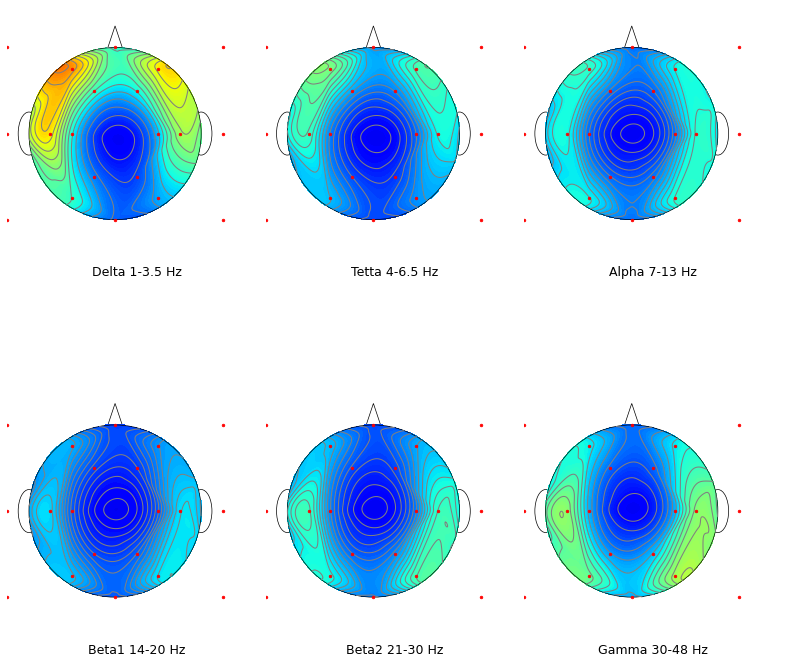
\includegraphics[width=\linewidth]{image_2022-05-12_17-19-49.png}
\caption{Meditation}
\label{fig:false-color}
\end{figure}




\begin{figure}[htbp]
\centering
\fbox{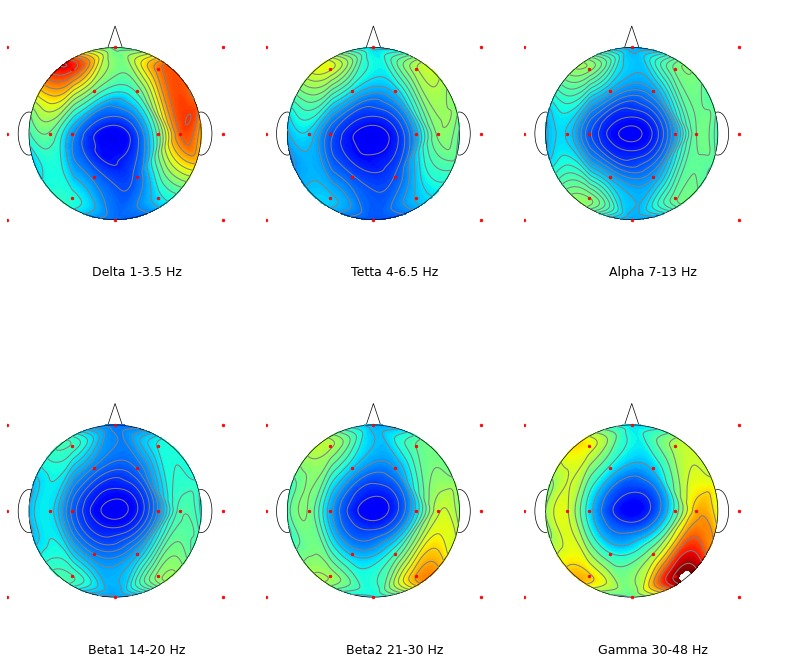
\includegraphics[width=\linewidth]{image_2022-05-12_17-18-54.png}}
\caption{Concentration}
\label{fig:false-color}
\end{figure}


From Fig.7 and Fig.8 we can conclude that all types of waves are increased in amplitude when a person is focused. Increased beta waves are expected to be higher during concentration, but not, for example, delta waves. Very high amplitudes of gamma waves suggest that the subject was stressed during the measurement, which is expected, given the pace of chosen games. 

\par We can also see that waves are situated asymmetrically. It can be explained by the fact that electrodes on one side are pressed more tightly so the contact is better which results in an asymmetrical picture.




\section{References}
\begin{enumerate}
    \item \href{https://www.sciencedirect.com/topics/agricultural-and-biological-sciences/brain-waves}{Science Direct - Brain Waves}
    \item \href{https://neuroplay.ru/#braincomputer}{NeuroPlayPro}
    \item \href{http://scholarpedia.org/article/Hilbert_transform_for_brain_waves}{Hilbert Transform}
    \item \href{https://en.wikipedia.org/wiki/Shapiro-Wilk_test}{Shapiro–Wilk test}
    \item \href{https://en.wikipedia.org/wiki/Multiple_comparisons_problem}{Multiple comparisons problem}
    \item \href{https://en.wikipedia.org/wiki/Student's_t-test}{T-test}
\end{enumerate}

\newpage

\section{Supplemental figures}

\begin{figure}[htbp]
\centering
\fbox{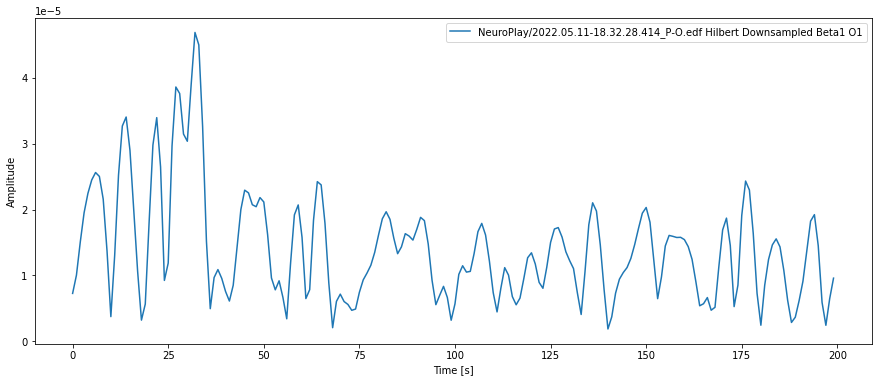
\includegraphics[width=\linewidth]{image_2022-05-12_16-22-11.png}}
\caption{Hilbert Downsampling on a signal}
\label{fig:false-color}
\end{figure}

\begin{figure}[htbp]
\centering
\fbox{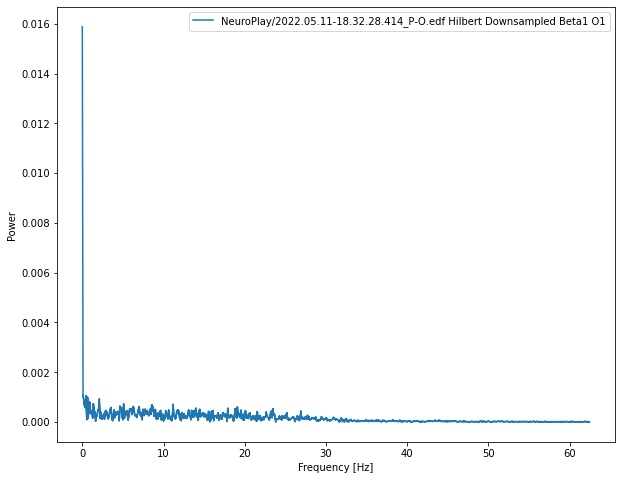
\includegraphics[width=\linewidth]{image_2022-05-12_16-22-11(1).png}}
\caption{Hilbert Downsampling on a spectrum}
\label{fig:false-color}
\end{figure}



\begin{figure}[htbp]
\centering
\fbox{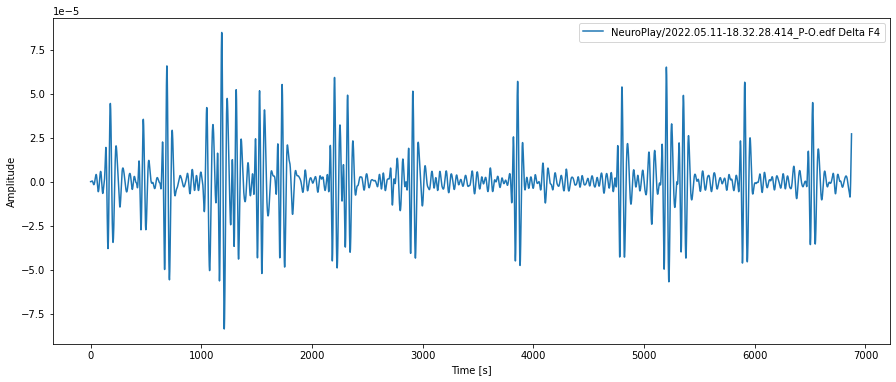
\includegraphics[width=\linewidth]{image_2022-05-12_17-32-34(1).png}}
\caption{Signal from a single electrode with open eyes}
\label{fig:false-color}
\end{figure}

\begin{figure}[htbp]
\centering
\fbox{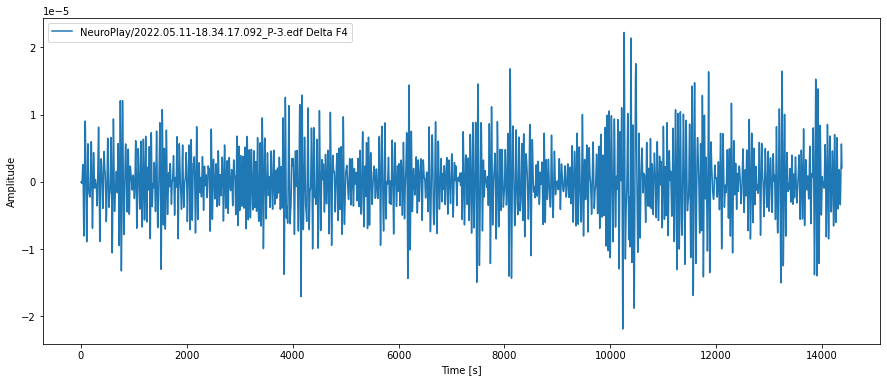
\includegraphics[width=\linewidth]{image_2022-05-12_17-32-52(1).png}}
\caption{Signal from a single electrode with closed eyes}
\label{fig:false-color}
\end{figure}






\end{document}
